\documentclass[11pt]{article}
\usepackage[margin=1in]{geometry}
\usepackage{amsmath,amssymb,amsthm}
\usepackage{booktabs}
\usepackage{multirow}
\usepackage{etoolbox}
\AtBeginEnvironment{table}{\small}
\usepackage{graphicx}
\usepackage[authoryear,round]{natbib}
\usepackage[hidelinks]{hyperref}

\newtheorem{proposition}{Proposition}
\theoremstyle{remark}
\newtheorem{remark}{Remark}

\newcommand{\E}{\mathbb{E}}

\title{Randomized Assignment-Based Anticlustering\\for Experiments with Many Arms}
\author{Gaurav Sood}
\date{\today}

\begin{document}
\maketitle

\begin{abstract}
Experiments with many arms suffer more chance imbalance on baseline
covariates, and the designs that remove it were built for two or a few
arms. Assignment-based anticlustering (ABA) splits units into equal groups
that are as alike as possible and scales to millions of units, but it is
deterministic. Jittering the sort that defines its batches and shuffling the
group labels make it a randomized design: every unit has probability $1/K$
of each arm, contrasts are unbiased, and the randomization test that
redraws the design is exact. We show that each ABA step is the greedy
allocation of the multi-arm adaptive design ARMM, computed by an assignment
problem in $O(K^3)$ rather than by scoring all $K!$ allocations; that without
jitter the arms are matched on the Mahalanobis norm to within its range
divided by the arm size; that one draw costs time and memory linear in the
number of units; and that rerandomization at a fixed acceptance rate loses
its gain as arms are added. In simulations with 4 to 50 arms, randomized ABA
balanced covariate means better than every other design whose cost is
linear in the number of units, including sequential covariate-adaptive
randomization, by a factor that grew with the number of arms. Balancing
means alone left omitted squares less balanced than complete randomization;
run on the covariates and their squares, randomized ABA gave the smallest
error and the most power for a nonlinear outcome in nearly every setting,
with exact size. With two arms, local search balanced better.
\end{abstract}

\section{Introduction}

Experiments increasingly compare many arms at once. A megastudy of gym
attendance tested 54 interventions on 61{,}293 people \citep{milkman2021};
platform experiments routinely split users across dozens of variants. Chance
imbalance on baseline covariates grows with the number of arms: under
complete randomization the summed squared imbalance across $K$ arms on $p$
whitened covariates is about $(K-1)p$, so the worst pair of arms is likely to
differ noticeably on something.

The designs that remove chance imbalance were built for two arms or a few.
Rerandomization \citep{morgan2012,li2018} draws complete randomizations until
one passes a balance threshold; with many arms the criterion has $(K-1)p$
degrees of freedom and, as Section~\ref{sec:theory} shows, a fixed
acceptance rate buys less and less. Covariate-adaptive randomization assigns
units one at a time toward the arm that most reduces imbalance
\citep{pocock1975,hu2012}; \citet{qin2024} balance the Mahalanobis distance
for two arms, and \citet{yang2023} extend this to $K$ arms by scoring all
$K!$ allocations of each block of $K$ units, which stops being feasible near
$K = 10$. \citet{zhang2023} gives a sequential procedure for any number of
arms and any feature map, with $O(1)$ imbalance; it scores $K$ options per
unit. Anticlustering \citep{papenberg2021,papenberg2026} splits units into
equal groups that are as alike as possible; its exchange heuristics cost
$O(N^2 p)$ per pass. \citet{baumann2026} introduce assignment-based
anticlustering (ABA), which scales to millions of units and hundreds of
thousands of groups and beats exchange heuristics on the anticlustering
objective when groups are many. ABA is deterministic, and its authors use it
for cross-validation folds, mini-batches and sample batching, not
experiments.

This note makes ABA a randomized design. Two changes suffice: noise in the
sort that defines ABA's batches, so that the partition itself is random, and
a uniform shuffle of the group labels. The result is a design in which every
unit has probability $1/K$ of each arm, the difference in means between any
two arms is unbiased, and the randomization test that redraws the design is
exact. We characterize what the design balances, what it costs, and what the
noise buys, and we compare it with complete randomization, blocking on an
index, rerandomization, sequential covariate-adaptive randomization, exchange
anticlustering and ARMM at 4 to 50 arms.

\section{The design}\label{sec:design}

Let $x_1, \dots, x_N \in \mathbb{R}^p$ be the covariates and $K$ the number
of arms, with $N = Km$. Whiten the covariates, $w_i = L^{-1}(x_i - \bar x)$
with $LL^\top$ the sample covariance, so that Euclidean distance on $w$ is
Mahalanobis distance on $x$. Draw one assignment as follows.
\begin{enumerate}
\item Compute the sort key $s_i = \|w_i\|^2 \exp(\sigma \varepsilon_i)$ with
  $\varepsilon_i$ independent standard normal and jitter $\sigma \ge 0$.
\item Sort units by $s_i$, largest first, and cut the list into $m$
  \emph{shells} of $K$ consecutive units.
\item Give the first shell one unit per group. For each later shell, assign
  its $K$ units one per group by the assignment that maximizes the total
  squared distance between each unit and its group's current centroid,
  solved exactly by the Hungarian or Jonker--Volgenant algorithm
  \citep{jonker1987}; then update the centroids.
\item Relabel the groups by a uniform random permutation of $\{1, \dots, K\}$.
\end{enumerate}
Steps 2 and 3 are ABA \citep{baumann2026}. Placing far-out units into the
group whose centroid is farthest from them pulls every centroid toward the
overall mean; giving each group one unit per shell matches the groups on the
distribution of distance from the centre. With $\sigma = 0$ the partition is
fixed and only step 4 is random. As $\sigma \to \infty$ the sort order
becomes a uniformly random permutation; by
Proposition~\ref{prop:step}, the design is then ARMM \citep{yang2023} with its
biased coin set to certainty, computed by an assignment problem instead of an
enumeration of $K!$ allocations.

\section{Properties}\label{sec:theory}

\begin{proposition}[Validity]\label{prop:valid}
For any covariates and any $\sigma$, the distribution of the assignment
$z = (z_1, \dots, z_N)$ is invariant under permutations of the arm labels.
Hence (i) $\Pr(z_i = g) = 1/K$ for every unit and arm; (ii) for any arms $a
\ne b$, the difference in means $\hat\tau_{ab} = m^{-1}\sum_i
(\mathbf{1}\{z_i = a\} - \mathbf{1}\{z_i = b\}) Y_i$ is unbiased for the
finite-population contrast $N^{-1}\sum_i \{Y_i(a) - Y_i(b)\}$; and (iii)
under the sharp null of no effect, the randomization test that compares the
observed statistic with its values on $D$ fresh draws of the design, with
p-value $(1 + \#\{|T_d| \ge |T_{\mathrm{obs}}|\})/(1 + D)$, satisfies
$\Pr(p \le \alpha) \le \alpha$.
\end{proposition}

\begin{proof}
Write $z = \pi \circ \zeta$, where $\zeta$ is the partition from steps 1--3
and $\pi$ is the uniform permutation of step 4, drawn independently. For any
fixed permutation $\rho$, $\rho \circ \pi$ is again uniform and independent
of $\zeta$, so $\rho \circ z$ has the distribution of $z$. Part (i) follows
because $\Pr(z_i = g) = \Pr(\pi(\zeta_i) = g) = 1/K$. Every arm has exactly
$m$ units, so $\E\,\hat\tau_{ab} = m^{-1}\sum_i \{\Pr(z_i = a) Y_i(a) -
\Pr(z_i = b) Y_i(b)\}$, which is (ii). Under the sharp null the outcomes do
not depend on $z$, so the observed and the $D$ reference draws are
independent and identically distributed draws from the design, and so are
their statistics. The rank of the observed statistic among the $1 + D$ is
then uniform, with ties broken against rejection, which is (iii).
\end{proof}

Validity therefore needs only the label shuffle. The jitter is about power
and robustness: with $\sigma = 0$ the design has at most $K!$ distinct
assignments, and a pair of units either always or never shares an arm.

\begin{proposition}[Each shell is assigned optimally]\label{prop:step}
Let $S_g$ be the sum of $w_i$ over the $t \ge 1$ units already in group $g$,
and $S'_g$ the sum after the next shell is assigned. Step 3 chooses, among
all $K!$ one-to-one allocations of the shell to the groups, one that
minimizes $\sum_g \|S'_g - \bar S'\|^2$, where $\bar S' = K^{-1}\sum_g S'_g$.
This criterion is proportional to the mean over pairs of arms of the
squared Mahalanobis distance between their sums, the criterion ARMM
minimizes with its \texttt{mean} option.
\end{proposition}

\begin{proof}
All groups hold $t$ units, so the centroids are $c_g = S_g/t$. If the shell's
unit $u_g$ goes to group $g$, the step-3 objective is $\sum_g \|w_{u_g} -
c_g\|^2 = \sum_g \|w_{u_g}\|^2 + \sum_g \|c_g\|^2 - (2/t)\sum_g \langle S_g,
w_{u_g}\rangle$, and only the last sum depends on the allocation; step 3
minimizes it. On the other side, $\sum_g \|S'_g\|^2 = \sum_g \|S_g\|^2 +
\sum_g \|w_{u_g}\|^2 + 2 \sum_g \langle S_g, w_{u_g}\rangle$, and $\bar S'$
does not depend on the allocation, so $\sum_g \|S'_g - \bar S'\|^2 = \sum_g
\|S'_g\|^2 - K\|\bar S'\|^2$ is minimized by the same allocation. Finally,
$\sum_{g<h}\|S'_g - S'_h\|^2 = K \sum_g \|S'_g - \bar S'\|^2$.
\end{proof}

So the $K!$ enumeration that limits ARMM to a handful of arms is
unnecessary: the same greedy step is a linear assignment problem, solvable
in $O(K^3)$. ARMM randomizes by taking its best allocation with probability
$q = 0.75$ and another at random otherwise; randomized ABA always takes the
best allocation and randomizes through the order and the labels.

\begin{proposition}[Balance on the sort key]\label{prop:key}
Let $\sigma = 0$. For any two groups $g, h$ produced by steps 1--3,
\[
\Bigl|\frac1m \sum_{i: \zeta_i = g} \|w_i\|^2 - \frac1m \sum_{i: \zeta_i = h}
\|w_i\|^2\Bigr| \le \frac{\max_i \|w_i\|^2 - \min_i \|w_i\|^2}{m}.
\]
For $\sigma > 0$ the same bound holds with the jittered key $s_i$ in place of
$\|w_i\|^2$.
\end{proposition}

\begin{proof}
Each group receives exactly one unit from each shell. Let $u_t$ and $l_t$ be
the largest and smallest key in shell $t$. The difference of the two groups'
keys within shell $t$ is at most $u_t - l_t$, so the difference of their sums
is at most $\sum_t (u_t - l_t)$. Shells are consecutive in the sorted order,
so $l_t \ge u_{t+1}$, and the sum telescopes to at most $u_1 - l_m$.
\end{proof}

The key $\|w_i\|^2$ is the sum of the squared whitened covariates, so
Proposition~\ref{prop:key} balances the arms on one quadratic summary, the
trace of each arm's second-moment matrix, to order $1/m$. It does not balance
the squares one by one; for that the design is run on the covariates with
their squares appended, which Section~\ref{sec:results} evaluates.

\begin{proposition}[Cost]\label{prop:cost}
One draw of randomized ABA takes $O(Np^2 + p^3)$ time to whiten, $O(N \log
N)$ to sort, and, for each of the $m$ shells, $O(K^2 p)$ to form the cost
matrix and $O(K^3)$ to solve the assignment problem: $O(Np^2 + N \log N +
NK(K + p))$ in all. Beyond the $N \times p$ covariates it needs $O(N + Kp +
K^2)$ memory: the sort order, the group sums and one $K \times K$ cost
matrix.
\end{proposition}

The count is immediate from the steps. Table~\ref{tab:cost} sets it against
the other designs. Three comparisons matter. ARMM computes, with probability
$q$, the same step as randomized ABA (Proposition~\ref{prop:step}) but by
scoring every allocation; the R implementation also stores the $K! \times K$
table of permutations, about $3.6 \times 10^7$ entries at $K = 10$ and $6
\times 10^9$ at $K = 12$, so memory fails before time does. The exchange
method is quadratic in $N$ per pass, and versions that work from a distance
matrix also need $O(N^2)$ memory; \citet{baumann2026} report exchange
heuristics failing to finish within two hours on a million units where ABA
takes seconds, and a hierarchical variant of ABA that replaces $K^2$ by
$LK^{2/L}$ for $L$ levels. The sequential procedure of \citet{zhang2023} is
cheaper than randomized ABA in $K$, linear rather than quadratic, and, unlike
any batch design, can assign units as they arrive while holding only the arm
sums; randomized ABA needs every unit's covariates before it assigns any. The
claim for randomized ABA is therefore not speed in $K$ but balance at a cost
linear in $N$; Section~\ref{sec:results} measures the balance.

\begin{table}[t]
\centering
\caption{Cost of one draw. $N$ units, $K$ arms of $m = N/K$, $p$ covariates, $q$ balancing features, $\alpha$ the rerandomization acceptance rate. Memory excludes the covariates themselves.}
\label{tab:cost}
\begin{tabular}{lll}
\toprule
 & Time & Memory \\
Design &  &  \\
\midrule
Complete randomization & $O(N)$ & $O(N)$ \\
Blocked on an index & $O(Np^2 + N \log N)$ & $O(N)$ \\
Rerandomization & $O(Np/\alpha)$ expected & $O(N)$ per candidate \\
Sequential CAR & $O(NKq)$ & $O(Kq)$, streaming \\
ARMM & $O(m\,K!\,K^2 p)$ & $O(K!\,K)$ \\
Exchange, per pass & $O(N^2 p)$ & $O(Kp)$; $O(N^2)$ with distances \\
Randomized ABA & $O(Np^2 + N\log N + NK(K+p))$ & $O(N + Kp + K^2)$ \\
\bottomrule
\end{tabular}
\end{table}


\begin{proposition}[Rerandomization with many arms]\label{prop:rr}
Under complete randomization into $K$ arms of $m$ units, the imbalance $B =
\sum_g m \|\bar w_g\|^2$ is approximately $\chi^2_d$ with $d = (K-1)p$.
Accepting only draws with $B \le a_\alpha$, the $\alpha$ quantile of
$\chi^2_d$, leaves expected imbalance
$v_\alpha(d)\,\E B$ with $v_\alpha(d) = \Pr(\chi^2_{d+2} \le
a_\alpha)/\alpha$, and $v_\alpha(d) \to 1$ as $d \to \infty$ for fixed
$\alpha$.
\end{proposition}

\begin{proof}
The formula for $v_\alpha$ is that of \citet{morgan2012} with $d$ degrees of
freedom. For the limit, $\chi^2_d/d \to 1$ in probability, so $a_\alpha / d
\to 1$; conditional on $B \le a_\alpha$, $B/d$ lies below $a_\alpha/d$ and,
since $\Pr(B \le (1-\delta)d)/\alpha \to 0$ for every $\delta > 0$, above
$1 - \delta$ with probability tending to one.
\end{proof}

At $\alpha = 0.01$, $v$ is 0.30 at $K = 4, p = 5$ but 0.78 at $K = 50, p =
5$ and 0.88 at $K = 50, p = 20$. Holding balance fixed instead drives the
acceptance rate to zero exponentially in $d$ \citep{qin2024}.

\section{Comparison}\label{sec:results}

\paragraph{Setup.} We compare designs at $K \in \{4, 10, 20, 50\}$ arms, $m
\in \{10, 40\}$ units per arm ($N$ from 40 to 2{,}000) and $p \in \{5, 20\}$
independent standard normal covariates, with 20 covariate draws per cell. The
designs are complete randomization; blocking on the first principal component
(sort, cut into blocks of $K$, permute within blocks); rerandomization at 1
percent acceptance on the $K$-arm criterion of Proposition~\ref{prop:rr};
the sequential procedure of \citet{zhang2023} with allocation function (4.3)
and $K_0 = 3$, on the whitened covariates with an intercept; one pass of the
exchange method of anticlustering \citep{papenberg2021} from a random start;
ARMM \citep{yang2023} through its R package, with units in random order (at
$K = 4$ only, on 10 draws per cell, and not at $m = 40, p = 20$, where it
takes about 15 minutes per cell); and randomized ABA with $\sigma = 1$. The
sequential procedure and randomized ABA are also run on the covariates with
their squares appended, and ABA with $\sigma = 0$ shows what the jitter does.
Each design draws 400 assignments per cell. The outcome has a linear part, a
quadratic part (squares and pairwise products of three covariates) and
noise, each of variance one. For the contrast between arms 1 and 2 we report
imbalance on the covariates and on their squares, both relative to complete
randomization; the mean squared error of the difference in means; the 95th
percentile, over draws of an unmeasured standard normal covariate, of the
OLS estimator's squared error relative to its value under exact balance;
and the size and power of the randomization test, at an effect of 1.96
standard errors of the complete-randomization difference in means.
Table~\ref{tab:many} reports $m = 40$ at $K = 4$ and $50$, and Figure~\ref{fig:many} all cells.

\begin{table}[t]
\centering
\caption{Many arms, $m = 40$ units per arm, $K = 4$ and $50$. Imbalance, on the covariates and on their squares, and MSE of the difference in means are ratios to complete randomization in the same draw. Tail is the 95th percentile of OLS error over an unmeasured covariate, relative to exact balance. Power and size are for the randomization test of the difference in means.}
\label{tab:many}
\begin{tabular}{lllrrrrrr}
\toprule
 &  &  & Imbalance & Imbalance sq. & Tail & MSE & Power & Size \\
K & p & Design &  &  &  &  &  &  \\
\midrule
\multirow[t]{19}{*}{4} & \multirow[t]{10}{*}{5} & complete & 1.000 & 1.000 & 1.27 & 1.00 & 0.48 & 0.05 \\
 &  & rerandomization & 0.298 & 1.015 & 1.24 & 0.85 & 0.55 & 0.05 \\
 &  & blocked & 0.819 & 0.915 & 1.29 & 0.95 & 0.51 & 0.05 \\
 &  & sequential CAR & 0.043 & 1.033 & 1.23 & 0.80 & 0.59 & 0.05 \\
 &  & sequential CAR, + sq. & 0.076 & 0.098 & 1.24 & 0.68 & 0.66 & 0.05 \\
 &  & exchange & 0.002 & 1.044 & 1.23 & 0.80 & 0.59 & 0.05 \\
 &  & ARMM & 0.062 & 1.042 & 1.23 & 0.85 & 0.57 & 0.05 \\
 &  & randomized ABA & 0.014 & 1.009 & 1.23 & 0.77 & 0.60 & 0.05 \\
 &  & randomized ABA, + sq. & 0.027 & 0.035 & 1.24 & 0.65 & 0.68 & 0.05 \\
 &  & ABA, no jitter & 0.006 & 0.884 & 2.61 & 0.62 & 0.00 & 0.00 \\
\cline{2-9}
 & \multirow[t]{9}{*}{20} & complete & 1.000 & 1.000 & 1.42 & 1.00 & 0.49 & 0.05 \\
 &  & rerandomization & 0.587 & 1.000 & 1.34 & 0.88 & 0.53 & 0.05 \\
 &  & blocked & 0.964 & 0.984 & 1.45 & 0.98 & 0.48 & 0.04 \\
 &  & sequential CAR & 0.131 & 0.998 & 1.26 & 0.78 & 0.56 & 0.05 \\
 &  & sequential CAR, + sq. & 0.242 & 0.261 & 1.29 & 0.70 & 0.63 & 0.05 \\
 &  & exchange & 0.034 & 1.003 & 1.25 & 0.74 & 0.61 & 0.05 \\
 &  & randomized ABA & 0.101 & 1.012 & 1.26 & 0.77 & 0.57 & 0.05 \\
 &  & randomized ABA, + sq. & 0.196 & 0.209 & 1.28 & 0.69 & 0.64 & 0.06 \\
 &  & ABA, no jitter & 0.079 & 0.928 & 2.61 & 0.62 & 0.00 & 0.00 \\
\cline{1-9} \cline{2-9}
\multirow[t]{18}{*}{50} & \multirow[t]{9}{*}{5} & complete & 1.000 & 1.000 & 1.13 & 1.00 & 0.49 & 0.05 \\
 &  & rerandomization & 0.777 & 1.002 & 1.13 & 0.97 & 0.50 & 0.05 \\
 &  & blocked & 0.803 & 0.940 & 1.13 & 0.92 & 0.54 & 0.05 \\
 &  & sequential CAR & 0.062 & 1.008 & 1.14 & 0.75 & 0.62 & 0.05 \\
 &  & sequential CAR, + sq. & 0.110 & 0.142 & 1.13 & 0.65 & 0.69 & 0.05 \\
 &  & exchange & 0.001 & 1.047 & 1.13 & 0.77 & 0.62 & 0.05 \\
 &  & randomized ABA & 0.004 & 1.444 & 1.13 & 0.83 & 0.57 & 0.05 \\
 &  & randomized ABA, + sq. & 0.008 & 0.009 & 1.13 & 0.59 & 0.72 & 0.05 \\
 &  & ABA, no jitter & 0.001 & 1.180 & 1.38 & 0.78 & 0.53 & 0.05 \\
\cline{2-9}
 & \multirow[t]{9}{*}{20} & complete & 1.000 & 1.000 & 1.14 & 1.00 & 0.51 & 0.05 \\
 &  & rerandomization & 0.884 & 1.000 & 1.14 & 1.01 & 0.49 & 0.05 \\
 &  & blocked & 0.951 & 0.993 & 1.14 & 1.01 & 0.48 & 0.05 \\
 &  & sequential CAR & 0.193 & 1.001 & 1.14 & 0.81 & 0.59 & 0.05 \\
 &  & sequential CAR, + sq. & 0.312 & 0.339 & 1.14 & 0.75 & 0.64 & 0.05 \\
 &  & exchange & 0.019 & 1.024 & 1.13 & 0.74 & 0.62 & 0.05 \\
 &  & randomized ABA & 0.026 & 1.105 & 1.13 & 0.80 & 0.59 & 0.05 \\
 &  & randomized ABA, + sq. & 0.045 & 0.050 & 1.13 & 0.61 & 0.69 & 0.05 \\
 &  & ABA, no jitter & 0.016 & 1.040 & 1.37 & 0.76 & 0.54 & 0.05 \\
\cline{1-9} \cline{2-9}
\bottomrule
\end{tabular}
\end{table}


\begin{figure}[t]
\centering
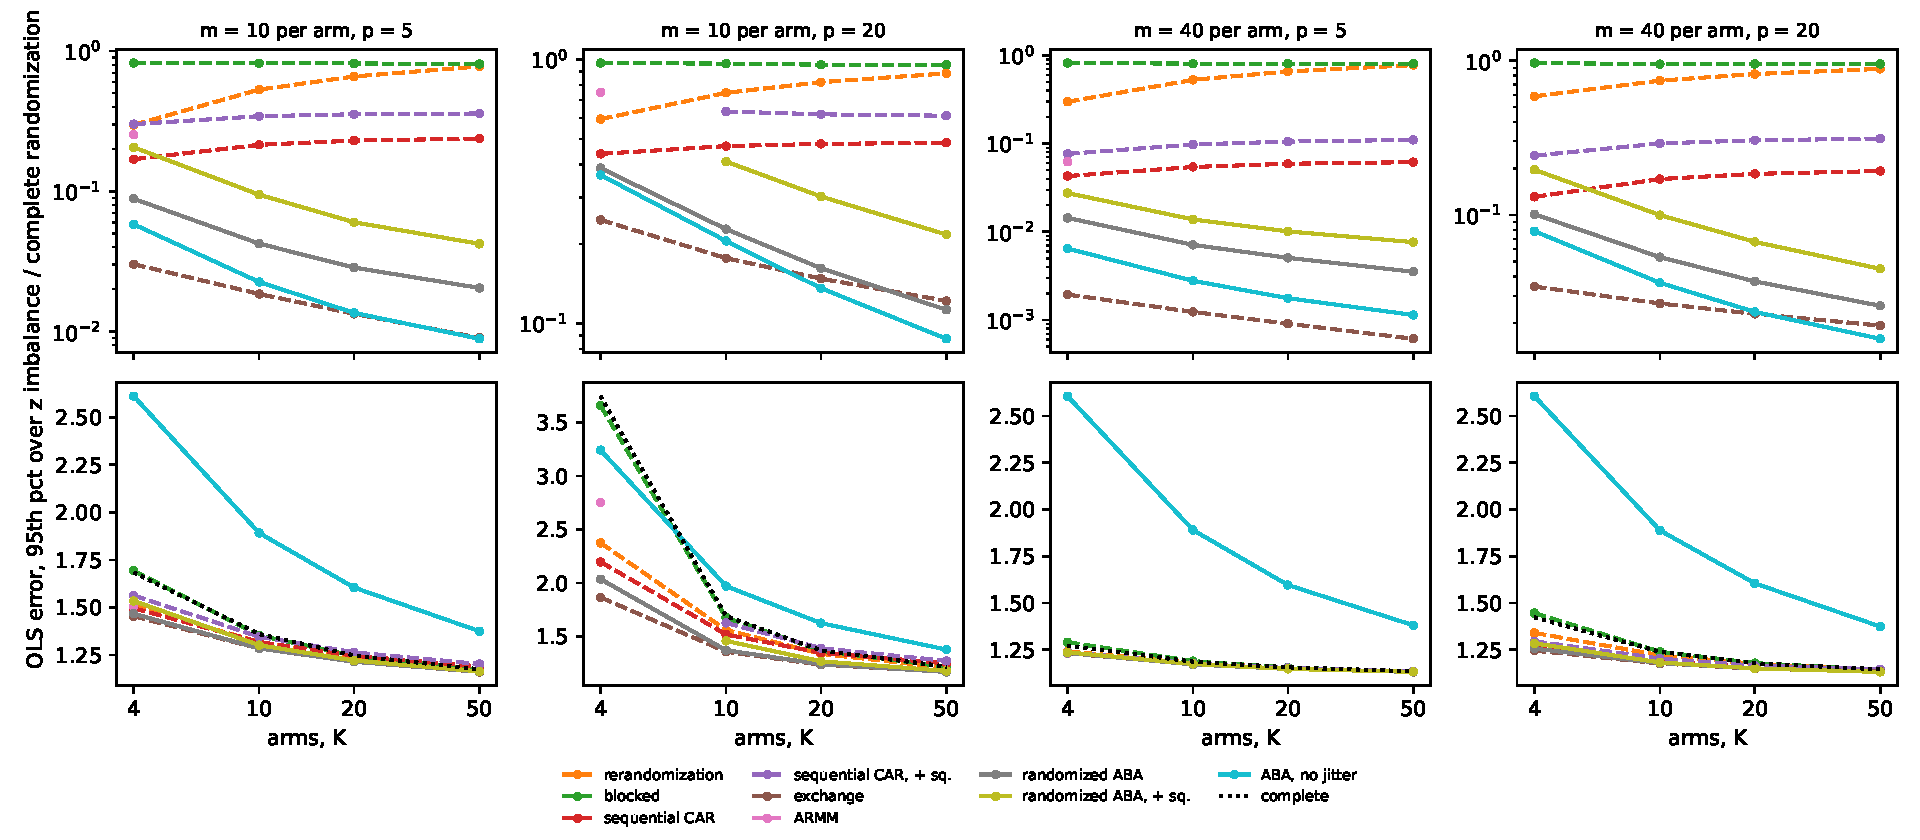
\includegraphics[width=\textwidth]{fig_many_arms.pdf}
\caption{Imbalance relative to complete randomization (top, log scale) and
the 95th percentile of OLS error over an unmeasured covariate (bottom),
against the number of arms. Each panel is one combination of units per arm
$m$ and covariates $p$.}
\label{fig:many}
\end{figure}

\paragraph{Balance on the covariates.} Among designs whose cost is linear in
$N$, randomized ABA balances best in every cell, and its lead grows with $K$.
At $m = 40$ and $p = 5$ its imbalance is 1.4 percent of complete
randomization's at $K = 4$ and 0.4 percent at $K = 50$; the sequential
procedure's is 4.3 and 6.2 percent, ARMM's 6.2 percent at $K = 4$. The
sequential procedure assigns each unit with probability bounded away from
zero for every arm, so its imbalance stays at a fixed multiple of the noise
floor as arms are added; randomized ABA's improves, because more arms mean
wider shells. Rerandomization fades as Proposition~\ref{prop:rr} predicts,
from 0.30 at $K = 4$ to 0.78 at $K = 50$ ($p = 5$); blocking on one index
removes under a fifth of the imbalance. The exchange method, quadratic in
$N$, balances means better still, by a factor of 1.4 to 7.

\paragraph{Omitted squares.} Balance on the covariates does not carry over
to their squares. Randomized ABA on the covariates alone leaves the squares
less balanced than complete randomization does, increasingly so with $K$: 1.44
times at $K = 50$, $m = 40$, $p = 5$. Putting the squares into the design
fixes this: at $m = 40$, randomized ABA on covariates and squares cuts
imbalance on the squares to between 0.9 and 21 percent of complete
randomization's, against 10 to 34 percent for the sequential procedure on the
same features, and except at $K = 4, p = 20$ it still balances the
covariates better than the sequential procedure on the covariates alone.

\paragraph{Estimation and power.} For the outcome with a quadratic part,
randomized ABA on covariates and squares has the smallest mean squared error
of the difference in means among designs with a usable test in every cell
but one, 59 to 69 percent of complete randomization's at $m = 40$, and the
most power, 0.64 to 0.72 against 0.63 to 0.69 for the sequential procedure on
the same features and 0.48 to 0.51 for complete randomization. (ABA without
jitter has lower error at $K = 4$, but its test cannot reject.) The randomization tests held their
size: the rejection rate under the null averaged 0.048 to 0.052 for every
randomized design. Over an unmeasured covariate, every randomized design's OLS tail is
at or slightly below complete randomization's.

\paragraph{The jitter.} With $\sigma = 0$ the partition is fixed and only
the labels are random. At $K = 4$ that leaves 24 assignments, too few for
the randomization test to reject at 5 percent, and the tail of OLS error over
an unmeasured covariate is 2.6 times the exact-balance value against 1.2 for
the jittered design. Table~\ref{tab:jitter} varies $\sigma$. A little jitter
($\sigma = 0.1$ to $0.3$) restores the tail while keeping almost all of the
balance. At $\sigma \ge 1$ the root mean square gap between co-assignment
probabilities and complete randomization's is within about 0.01 of complete
randomization's own Monte Carlo floor, though the most co-assigned pair still
shares an arm 1.2 to 4.5 times as often. At $\sigma = 10$, effectively a
random order, imbalance is still 1.7 to 7 percent of complete
randomization's: most of the balance comes from the assignment step, and the
sort adds a factor of 1.7 to 2.4 at $\sigma = 1$ and 3 to 6 at $\sigma = 0$.

\begin{table}[t]
\centering
\caption{Randomized ABA by jitter $\sigma$, $p = 5$. Imbalance is relative to complete randomization; co-assignment is the probability that two units share an arm, whose RMS gap from complete randomization's value includes Monte Carlo noise of about complete randomization's own gap.}
\label{tab:jitter}
\begin{tabular}{lllrrrr}
\toprule
 &  &  & Imbalance & OLS tail & Max co-assignment & RMS gap \\
K & m & Design &  &  &  &  \\
\midrule
\multirow[t]{14}{*}{10} & \multirow[t]{7}{*}{10} & complete & 1.000 & 1.360 & 0.147 & 0.014 \\
 &  & jitter 0 & 0.022 & 1.900 & 1.000 & 0.287 \\
 &  & jitter 0.1 & 0.024 & 1.302 & 0.674 & 0.044 \\
 &  & jitter 0.3 & 0.027 & 1.290 & 0.407 & 0.031 \\
 &  & jitter 1 & 0.043 & 1.285 & 0.336 & 0.026 \\
 &  & jitter 3 & 0.062 & 1.282 & 0.286 & 0.026 \\
 &  & jitter 10 & 0.071 & 1.286 & 0.283 & 0.025 \\
\cline{2-7}
 & \multirow[t]{7}{*}{40} & complete & 1.000 & 1.185 & 0.166 & 0.015 \\
 &  & jitter 0 & 0.003 & 1.884 & 1.000 & 0.297 \\
 &  & jitter 0.1 & 0.003 & 1.175 & 0.549 & 0.020 \\
 &  & jitter 0.3 & 0.003 & 1.174 & 0.290 & 0.017 \\
 &  & jitter 1 & 0.007 & 1.169 & 0.205 & 0.016 \\
 &  & jitter 3 & 0.014 & 1.173 & 0.184 & 0.016 \\
 &  & jitter 10 & 0.017 & 1.173 & 0.185 & 0.016 \\
\cline{1-7} \cline{2-7}
\multirow[t]{7}{*}{50} & \multirow[t]{7}{*}{10} & complete & 1.000 & 1.174 & 0.054 & 0.007 \\
 &  & jitter 0 & 0.009 & 1.384 & 1.000 & 0.133 \\
 &  & jitter 0.1 & 0.009 & 1.169 & 0.675 & 0.016 \\
 &  & jitter 0.3 & 0.010 & 1.165 & 0.334 & 0.011 \\
 &  & jitter 1 & 0.021 & 1.162 & 0.241 & 0.010 \\
 &  & jitter 3 & 0.035 & 1.164 & 0.181 & 0.009 \\
 &  & jitter 10 & 0.041 & 1.166 & 0.182 & 0.010 \\
\cline{1-7} \cline{2-7}
\bottomrule
\end{tabular}
\end{table}


\paragraph{Two arms.} With two arms randomized ABA is not the best design.
At $N = 120$, greedy pair-switching \citep{krieger2019}, which swaps units
until no swap improves balance, balances means 5 to 14 times better, and on
covariates with squares it matches or beats randomized ABA in power (0.69
against 0.63 at $p = 20$). At $p = 20$ and $30$ the sequential procedure
also balances means better than randomized ABA and, with squares, has more
power. Splitting units into many small groups by
randomized ABA and treating half the groups does worse than randomized ABA
with two groups directly. Randomized ABA's case is many arms (Table~\ref{tab:two}).

\begin{table}[t]
\centering
\caption{Two arms, $N = 120$; columns as in Table~\ref{tab:many}.}
\label{tab:two}
\begin{tabular}{llrrrrrr}
\toprule
 &  & Imbalance & Imbalance sq. & Tail & MSE & Power & Size \\
p & Design &  &  &  &  &  &  \\
\midrule
\multirow[t]{9}{*}{5} & complete & 1.000 & 1.000 & 1.31 & 1.00 & 0.51 & 0.05 \\
 & rerandomization & 0.077 & 0.995 & 1.26 & 0.81 & 0.59 & 0.05 \\
 & sequential CAR & 0.023 & 0.985 & 1.26 & 0.80 & 0.60 & 0.05 \\
 & sequential CAR, + sq. & 0.041 & 0.051 & 1.27 & 0.61 & 0.70 & 0.05 \\
 & randomized ABA & 0.018 & 0.938 & 1.26 & 0.74 & 0.62 & 0.05 \\
 & randomized ABA, + sq. & 0.035 & 0.043 & 1.27 & 0.60 & 0.72 & 0.05 \\
 & greedy switching & 0.001 & 1.020 & 1.26 & 0.78 & 0.62 & 0.05 \\
 & greedy switching, + sq. & 0.003 & 0.004 & 1.27 & 0.59 & 0.72 & 0.05 \\
 & randomized ABA, pairs & 0.246 & 1.381 & 1.29 & 0.93 & 0.53 & 0.05 \\
\cline{1-8}
\multirow[t]{9}{*}{20} & complete & 1.000 & 1.000 & 1.54 & 1.00 & 0.49 & 0.05 \\
 & rerandomization & 0.362 & 1.015 & 1.36 & 0.85 & 0.57 & 0.05 \\
 & sequential CAR & 0.070 & 1.006 & 1.29 & 0.76 & 0.60 & 0.05 \\
 & sequential CAR, + sq. & 0.139 & 0.152 & 1.33 & 0.63 & 0.68 & 0.05 \\
 & randomized ABA & 0.122 & 1.008 & 1.30 & 0.80 & 0.58 & 0.05 \\
 & randomized ABA, + sq. & 0.237 & 0.252 & 1.35 & 0.69 & 0.63 & 0.05 \\
 & greedy switching & 0.022 & 1.000 & 1.28 & 0.75 & 0.59 & 0.05 \\
 & greedy switching, + sq. & 0.053 & 0.060 & 1.32 & 0.61 & 0.69 & 0.05 \\
 & randomized ABA, pairs & 0.569 & 1.147 & 1.43 & 0.94 & 0.52 & 0.05 \\
\cline{1-8}
\multirow[t]{9}{*}{30} & complete & 1.000 & 1.000 & 1.73 & 1.00 & 0.46 & 0.05 \\
 & rerandomization & 0.455 & 0.994 & 1.46 & 0.82 & 0.55 & 0.05 \\
 & sequential CAR & 0.103 & 0.992 & 1.33 & 0.75 & 0.58 & 0.05 \\
 & sequential CAR, + sq. & 0.201 & 0.209 & 1.41 & 0.61 & 0.66 & 0.05 \\
 & randomized ABA & 0.187 & 0.993 & 1.35 & 0.76 & 0.57 & 0.05 \\
 & randomized ABA, + sq. & 0.349 & 0.359 & 1.46 & 0.66 & 0.61 & 0.05 \\
 & greedy switching & 0.039 & 0.991 & 1.30 & 0.73 & 0.57 & 0.05 \\
 & greedy switching, + sq. & 0.097 & 0.104 & 1.39 & 0.58 & 0.69 & 0.05 \\
 & randomized ABA, pairs & 0.660 & 1.087 & 1.57 & 0.92 & 0.48 & 0.05 \\
\cline{1-8}
\bottomrule
\end{tabular}
\end{table}


\section{Discussion}

Randomized ABA is ABA with two random steps added, and the steps are what make
it a design: the label shuffle gives exact randomization inference, and the
jitter gives the partition enough variation for the test to have power and
for an unmeasured covariate to be balanced as well as under complete
randomization. ABA's assignment step turns out to be the greedy allocation of
ARMM, so the many-arm covariate-adaptive designs and the anticlustering
literature have been computing the same thing by different routes; the
assignment problem is the cheap one.

The practical recommendation is to run randomized ABA on the covariates and
their squares whenever all units are known before assignment and the arms
are more than a handful. When units arrive one at a time, the sequential
procedure of \citet{zhang2023} is the tool, at some cost in balance. With two
arms and a few hundred units, local search such as greedy pair-switching
balances better. The exchange method balances means better than randomized
ABA at every size we tried but is quadratic in $N$, which matters at the
scales where ABA was built to run.

The comparison has limits. Covariates are Gaussian and effects constant; one
outcome model drives the error and power results; $N$ stops at 2{,}000,
below the scale at which the cost differences bite; and ARMM appears only at
four arms.


\bibliographystyle{plainnat}
\bibliography{refs}

\end{document}
